\documentclass[twoside]{book}

% Packages required by doxygen
\usepackage{fixltx2e}
\usepackage{calc}
\usepackage{doxygen}
\usepackage[export]{adjustbox} % also loads graphicx
\usepackage{graphicx}
\usepackage[utf8]{inputenc}
\usepackage{makeidx}
\usepackage{multicol}
\usepackage{multirow}
\PassOptionsToPackage{warn}{textcomp}
\usepackage{textcomp}
\usepackage[nointegrals]{wasysym}
\usepackage[table]{xcolor}

% Font selection
\usepackage[T1]{fontenc}
\usepackage[scaled=.90]{helvet}
\usepackage{courier}
\usepackage{amssymb}
\usepackage{sectsty}
\renewcommand{\familydefault}{\sfdefault}
\allsectionsfont{%
  \fontseries{bc}\selectfont%
  \color{darkgray}%
}
\renewcommand{\DoxyLabelFont}{%
  \fontseries{bc}\selectfont%
  \color{darkgray}%
}
\newcommand{\+}{\discretionary{\mbox{\scriptsize$\hookleftarrow$}}{}{}}

% Page & text layout
\usepackage{geometry}
\geometry{%
  a4paper,%
  top=2.5cm,%
  bottom=2.5cm,%
  left=2.5cm,%
  right=2.5cm%
}
\tolerance=750
\hfuzz=15pt
\hbadness=750
\setlength{\emergencystretch}{15pt}
\setlength{\parindent}{0cm}
\setlength{\parskip}{3ex plus 2ex minus 2ex}
\makeatletter
\renewcommand{\paragraph}{%
  \@startsection{paragraph}{4}{0ex}{-1.0ex}{1.0ex}{%
    \normalfont\normalsize\bfseries\SS@parafont%
  }%
}
\renewcommand{\subparagraph}{%
  \@startsection{subparagraph}{5}{0ex}{-1.0ex}{1.0ex}{%
    \normalfont\normalsize\bfseries\SS@subparafont%
  }%
}
\makeatother

% Headers & footers
\usepackage{fancyhdr}
\pagestyle{fancyplain}
\fancyhead[LE]{\fancyplain{}{\bfseries\thepage}}
\fancyhead[CE]{\fancyplain{}{}}
\fancyhead[RE]{\fancyplain{}{\bfseries\leftmark}}
\fancyhead[LO]{\fancyplain{}{\bfseries\rightmark}}
\fancyhead[CO]{\fancyplain{}{}}
\fancyhead[RO]{\fancyplain{}{\bfseries\thepage}}
\fancyfoot[LE]{\fancyplain{}{}}
\fancyfoot[CE]{\fancyplain{}{}}
\fancyfoot[RE]{\fancyplain{}{\bfseries\scriptsize Generated by Doxygen }}
\fancyfoot[LO]{\fancyplain{}{\bfseries\scriptsize Generated by Doxygen }}
\fancyfoot[CO]{\fancyplain{}{}}
\fancyfoot[RO]{\fancyplain{}{}}
\renewcommand{\footrulewidth}{0.4pt}
\renewcommand{\chaptermark}[1]{%
  \markboth{#1}{}%
}
\renewcommand{\sectionmark}[1]{%
  \markright{\thesection\ #1}%
}

% Indices & bibliography
\usepackage{natbib}
\usepackage[titles]{tocloft}
\setcounter{tocdepth}{3}
\setcounter{secnumdepth}{5}
\makeindex

% Hyperlinks (required, but should be loaded last)
\usepackage{ifpdf}
\ifpdf
  \usepackage[pdftex,pagebackref=true]{hyperref}
\else
  \usepackage[ps2pdf,pagebackref=true]{hyperref}
\fi
\hypersetup{%
  colorlinks=true,%
  linkcolor=blue,%
  citecolor=blue,%
  unicode%
}

% Custom commands
\newcommand{\clearemptydoublepage}{%
  \newpage{\pagestyle{empty}\cleardoublepage}%
}

\usepackage{caption}
\captionsetup{labelsep=space,justification=centering,font={bf},singlelinecheck=off,skip=4pt,position=top}

%===== C O N T E N T S =====

\begin{document}

% Titlepage & ToC
\hypersetup{pageanchor=false,
             bookmarksnumbered=true,
             pdfencoding=unicode
            }
\pagenumbering{alph}
\begin{titlepage}
\vspace*{7cm}
\begin{center}%
{\Large Ghost \\[1ex]\large 0.\+1 }\\
\vspace*{1cm}
{\large Generated by Doxygen 1.8.14}\\
\end{center}
\end{titlepage}
\clearemptydoublepage
\pagenumbering{roman}
\tableofcontents
\clearemptydoublepage
\pagenumbering{arabic}
\hypersetup{pageanchor=true}

%--- Begin generated contents ---
\chapter{Namespace Index}
\section{Packages}
Here are the packages with brief descriptions (if available)\+:\begin{DoxyCompactList}
\item\contentsline{section}{\mbox{\hyperlink{namespaceAgency}{Agency}} \\*Documentation for \mbox{\hyperlink{namespaceAgency}{Agency}} }{\pageref{namespaceAgency}}{}
\item\contentsline{section}{\mbox{\hyperlink{namespaceArchitectures}{Architectures}} \\*Documentation for \mbox{\hyperlink{namespaceArchitectures}{Architectures}} }{\pageref{namespaceArchitectures}}{}
\item\contentsline{section}{\mbox{\hyperlink{namespacemain}{main}} \\*Documentation for the main file }{\pageref{namespacemain}}{}
\end{DoxyCompactList}

\chapter{Hierarchical Index}
\section{Class Hierarchy}
This inheritance list is sorted roughly, but not completely, alphabetically\+:\begin{DoxyCompactList}
\item Base\+Agent\begin{DoxyCompactList}
\item \contentsline{section}{Agency.\+Base\+Agent}{\pageref{classAgency_1_1BaseAgent}}{}
\end{DoxyCompactList}
\item Module\begin{DoxyCompactList}
\item \contentsline{section}{Architectures.\+Pytorch\+Tutorial\+D\+QN}{\pageref{classArchitectures_1_1PytorchTutorialDQN}}{}
\end{DoxyCompactList}
\item object\begin{DoxyCompactList}
\item \contentsline{section}{Agency.\+Replay\+Buffer}{\pageref{classAgency_1_1ReplayBuffer}}{}
\end{DoxyCompactList}
\end{DoxyCompactList}

\chapter{Class Index}
\section{Class List}
Here are the classes, structs, unions and interfaces with brief descriptions\+:\begin{DoxyCompactList}
\item\contentsline{section}{\mbox{\hyperlink{classAgency_1_1BaseAgent}{Agency.\+Base\+Agent}} \\*Documentation for \mbox{\hyperlink{classAgency_1_1BaseAgent}{Base\+Agent}} }{\pageref{classAgency_1_1BaseAgent}}{}
\item\contentsline{section}{\mbox{\hyperlink{classArchitectures_1_1PytorchTutorialDQN}{Architectures.\+Pytorch\+Tutorial\+D\+QN}} \\*Documentation for \mbox{\hyperlink{classArchitectures_1_1PytorchTutorialDQN}{Pytorch\+Tutorial\+D\+QN}} }{\pageref{classArchitectures_1_1PytorchTutorialDQN}}{}
\item\contentsline{section}{\mbox{\hyperlink{classAgency_1_1ReplayBuffer}{Agency.\+Replay\+Buffer}} \\*Documentation for \mbox{\hyperlink{classAgency_1_1ReplayBuffer}{Replay\+Buffer}} }{\pageref{classAgency_1_1ReplayBuffer}}{}
\end{DoxyCompactList}

\chapter{Namespace Documentation}
\hypertarget{namespaceAgency}{}\section{Agency Namespace Reference}
\label{namespaceAgency}\index{Agency@{Agency}}


Documentation for \mbox{\hyperlink{namespaceAgency}{Agency}}.  


\subsection*{Classes}
\begin{DoxyCompactItemize}
\item 
class \mbox{\hyperlink{classAgency_1_1BaseAgent}{Base\+Agent}}
\begin{DoxyCompactList}\small\item\em Documentation for \mbox{\hyperlink{classAgency_1_1BaseAgent}{Base\+Agent}}. \end{DoxyCompactList}\item 
class \mbox{\hyperlink{classAgency_1_1ReplayBuffer}{Replay\+Buffer}}
\begin{DoxyCompactList}\small\item\em Documentation for \mbox{\hyperlink{classAgency_1_1ReplayBuffer}{Replay\+Buffer}}. \end{DoxyCompactList}\end{DoxyCompactItemize}


\subsection{Detailed Description}
Documentation for \mbox{\hyperlink{namespaceAgency}{Agency}}. 

More details. 
\hypertarget{namespaceArchitectures}{}\section{Architectures Namespace Reference}
\label{namespaceArchitectures}\index{Architectures@{Architectures}}


Documentation for \mbox{\hyperlink{namespaceArchitectures}{Architectures}}.  


\subsection*{Classes}
\begin{DoxyCompactItemize}
\item 
class \mbox{\hyperlink{classArchitectures_1_1PytorchTutorialDQN}{Pytorch\+Tutorial\+D\+QN}}
\begin{DoxyCompactList}\small\item\em Documentation for \mbox{\hyperlink{classArchitectures_1_1PytorchTutorialDQN}{Pytorch\+Tutorial\+D\+QN}}. \end{DoxyCompactList}\end{DoxyCompactItemize}


\subsection{Detailed Description}
Documentation for \mbox{\hyperlink{namespaceArchitectures}{Architectures}}. 

More details. 
\hypertarget{namespacemain}{}\section{main Namespace Reference}
\label{namespacemain}\index{main@{main}}


Documentation for the main file.  


\subsection*{Functions}
\begin{DoxyCompactItemize}
\item 
def \mbox{\hyperlink{namespacemain_af3f5f1d2e9b06bf119f500dced42f536}{main}} (argv)
\begin{DoxyCompactList}\small\item\em Reads in several flags to pass it to the running app (pysc2). \end{DoxyCompactList}\end{DoxyCompactItemize}
\subsection*{Variables}
\begin{DoxyCompactItemize}
\item 
\mbox{\Hypertarget{namespacemain_a9e54bf13f9d353cfeb8aa9a5623dcf87}\label{namespacemain_a9e54bf13f9d353cfeb8aa9a5623dcf87}} 
\mbox{\hyperlink{namespacemain_a9e54bf13f9d353cfeb8aa9a5623dcf87}{F\+L\+A\+GS}} = flags.\+F\+L\+A\+GS
\begin{DoxyCompactList}\small\item\em contains hyperparameter input \end{DoxyCompactList}\end{DoxyCompactItemize}


\subsection{Detailed Description}
Documentation for the main file. 

\begin{DoxyVerb}__author__ = "Hendrik Vloet"
__copyright__ = "Copyright (C) 2018 Hendrik Vloet"
__license__ = "Public Domain"
__version__ = "1.0"
\end{DoxyVerb}


The main file serves only to read in hyperparemeters, construct architecture \& agent objects and finally run the agent with the agent.\+play() method 

\subsection{Function Documentation}
\mbox{\Hypertarget{namespacemain_af3f5f1d2e9b06bf119f500dced42f536}\label{namespacemain_af3f5f1d2e9b06bf119f500dced42f536}} 
\index{main@{main}!main@{main}}
\index{main@{main}!main@{main}}
\subsubsection{\texorpdfstring{main()}{main()}}
{\footnotesize\ttfamily def main.\+main (\begin{DoxyParamCaption}\item[{}]{argv }\end{DoxyParamCaption})}



Reads in several flags to pass it to the running app (pysc2). 

Flag Description
\begin{DoxyItemize}
\item learning\+\_\+rate, float\+: learning for the optimizer
\item gamma, float\+: Discount factor
\item batch\+\_\+size, unsigned int\+: Batch size of the samples durch experience replay
\item target\+\_\+update, unsigned int\+: Update Target network every N episodes
\item epochs, unsigned int\+: amount of episodes to train
\item memory\+\_\+size, unsigned int\+: capacity of the replay buffer
\item visualize, bool\+: set true for actual screen displaying
\item architecture, string\+: specifiy architecture/network-\/model to use
\item xy\+\_\+grid, unsigned int\+: \char`\"{}discretizes\char`\"{} the action spaces into NxN \mbox{[}x,y\mbox{]}-\/pairs
\item epsilon, unsigned int\+: the decay rate for the decaying epsilon greedy policy (epsilon $\sim$ decay\+Time)
\item map\+\_\+name, string\+: map/scenario to play
\item step\+\_\+multiplier, unsigned int\+: how many game steps per agent step 
\end{DoxyItemize}
\chapter{Class Documentation}
\hypertarget{classAgency_1_1BaseAgent}{}\section{Agency.\+Base\+Agent Class Reference}
\label{classAgency_1_1BaseAgent}\index{Agency.\+Base\+Agent@{Agency.\+Base\+Agent}}


Documentation for \mbox{\hyperlink{classAgency_1_1BaseAgent}{Base\+Agent}}.  


Inheritance diagram for Agency.\+Base\+Agent\+:\begin{figure}[H]
\begin{center}
\leavevmode
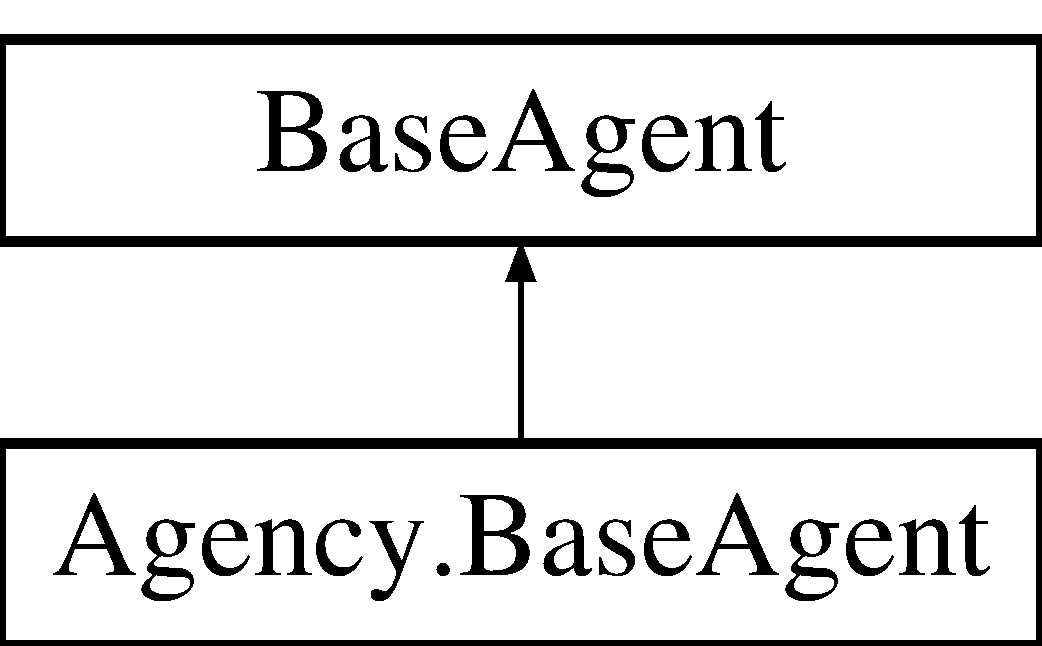
\includegraphics[height=2.000000cm]{classAgency_1_1BaseAgent}
\end{center}
\end{figure}
\subsection*{Public Member Functions}
\begin{DoxyCompactItemize}
\item 
\mbox{\Hypertarget{classAgency_1_1BaseAgent_a8000d3852f7eada76fd862a036e8c5ac}\label{classAgency_1_1BaseAgent_a8000d3852f7eada76fd862a036e8c5ac}} 
def {\bfseries \+\_\+\+\_\+init\+\_\+\+\_\+} (self, architecture, F\+L\+A\+GS, device=\char`\"{}cpu\char`\"{})
\item 
def \mbox{\hyperlink{classAgency_1_1BaseAgent_a901aab539081be07996dca97de2f2e06}{decide}} (self)
\item 
\mbox{\Hypertarget{classAgency_1_1BaseAgent_a1f7d1b84d919eb3d2ce9092ad2161d1b}\label{classAgency_1_1BaseAgent_a1f7d1b84d919eb3d2ce9092ad2161d1b}} 
def {\bfseries choose\+\_\+action} (self)
\item 
\mbox{\Hypertarget{classAgency_1_1BaseAgent_a06cd034442fe41432486654dfafa0937}\label{classAgency_1_1BaseAgent_a06cd034442fe41432486654dfafa0937}} 
def {\bfseries extract\+\_\+action} (self)
\item 
\mbox{\Hypertarget{classAgency_1_1BaseAgent_a59f2f9a055e2c145bc83f610e26b8096}\label{classAgency_1_1BaseAgent_a59f2f9a055e2c145bc83f610e26b8096}} 
def {\bfseries step} (self)
\item 
\mbox{\Hypertarget{classAgency_1_1BaseAgent_a663f1d2913fa6a467077a55ddf854dae}\label{classAgency_1_1BaseAgent_a663f1d2913fa6a467077a55ddf854dae}} 
def {\bfseries calc\+\_\+pseudo\+\_\+reward} (self)
\item 
\mbox{\Hypertarget{classAgency_1_1BaseAgent_adef4f441aa6cbd1f3bb2c85839b9f403}\label{classAgency_1_1BaseAgent_adef4f441aa6cbd1f3bb2c85839b9f403}} 
def {\bfseries optimize} (self)
\item 
\mbox{\Hypertarget{classAgency_1_1BaseAgent_a9cb7dd560c63c2fe8d1967568b6a82ed}\label{classAgency_1_1BaseAgent_a9cb7dd560c63c2fe8d1967568b6a82ed}} 
def {\bfseries print\+\_\+status} (self)
\item 
\mbox{\Hypertarget{classAgency_1_1BaseAgent_aa06a4883d4637c0fdfca1d8d37f94069}\label{classAgency_1_1BaseAgent_aa06a4883d4637c0fdfca1d8d37f94069}} 
def {\bfseries play} (self)
\end{DoxyCompactItemize}
\subsection*{Public Attributes}
\begin{DoxyCompactItemize}
\item 
\mbox{\Hypertarget{classAgency_1_1BaseAgent_aac02c4ec3cb8092b0658a5016ca34da5}\label{classAgency_1_1BaseAgent_aac02c4ec3cb8092b0658a5016ca34da5}} 
{\bfseries epsilon}
\item 
\mbox{\Hypertarget{classAgency_1_1BaseAgent_a0fd91f1d7a6e98d7a595a10cca3971f6}\label{classAgency_1_1BaseAgent_a0fd91f1d7a6e98d7a595a10cca3971f6}} 
{\bfseries total\+\_\+reward}
\item 
\mbox{\Hypertarget{classAgency_1_1BaseAgent_aa35d9fa21795e21339570f483d99b56c}\label{classAgency_1_1BaseAgent_aa35d9fa21795e21339570f483d99b56c}} 
{\bfseries memory}
\item 
\mbox{\Hypertarget{classAgency_1_1BaseAgent_a0bfa57fad07747f81f83d3e6f2c8a493}\label{classAgency_1_1BaseAgent_a0bfa57fad07747f81f83d3e6f2c8a493}} 
{\bfseries choice}
\item 
\mbox{\Hypertarget{classAgency_1_1BaseAgent_adcc438ca0e3c70602fc3fd8941380dfd}\label{classAgency_1_1BaseAgent_adcc438ca0e3c70602fc3fd8941380dfd}} 
{\bfseries action\+\_\+idx}
\item 
\mbox{\Hypertarget{classAgency_1_1BaseAgent_a72269503c3be981fe59c51e6f46563c2}\label{classAgency_1_1BaseAgent_a72269503c3be981fe59c51e6f46563c2}} 
{\bfseries action\+\_\+xy}
\item 
\mbox{\Hypertarget{classAgency_1_1BaseAgent_a806c86c1018317a32f8a2b297b465ff4}\label{classAgency_1_1BaseAgent_a806c86c1018317a32f8a2b297b465ff4}} 
{\bfseries action\+\_\+q\+\_\+values}
\item 
\mbox{\Hypertarget{classAgency_1_1BaseAgent_a9b17cee37319f16020cee6a23321c893}\label{classAgency_1_1BaseAgent_a9b17cee37319f16020cee6a23321c893}} 
{\bfseries x\+\_\+coord}
\item 
\mbox{\Hypertarget{classAgency_1_1BaseAgent_a41d5c1c526ff266223f9b2e0ad7cf1c7}\label{classAgency_1_1BaseAgent_a41d5c1c526ff266223f9b2e0ad7cf1c7}} 
{\bfseries y\+\_\+coord}
\item 
\mbox{\Hypertarget{classAgency_1_1BaseAgent_a7ac4296207527be00adc988fa95af709}\label{classAgency_1_1BaseAgent_a7ac4296207527be00adc988fa95af709}} 
{\bfseries pysc\+\_\+action}
\item 
\mbox{\Hypertarget{classAgency_1_1BaseAgent_ab1ef5401d902e7e79853793e386d80c5}\label{classAgency_1_1BaseAgent_ab1ef5401d902e7e79853793e386d80c5}} 
{\bfseries action}
\item 
\mbox{\Hypertarget{classAgency_1_1BaseAgent_a63134b494c76d05c1368abba3cefad16}\label{classAgency_1_1BaseAgent_a63134b494c76d05c1368abba3cefad16}} 
{\bfseries beacon}
\item 
\mbox{\Hypertarget{classAgency_1_1BaseAgent_ae35f3a8539b94d37bdd0e401f1fe8349}\label{classAgency_1_1BaseAgent_ae35f3a8539b94d37bdd0e401f1fe8349}} 
{\bfseries m\+\_\+x}
\item 
\mbox{\Hypertarget{classAgency_1_1BaseAgent_a4809237727e0865b7a47b0cd71525ef6}\label{classAgency_1_1BaseAgent_a4809237727e0865b7a47b0cd71525ef6}} 
{\bfseries m\+\_\+y}
\item 
\mbox{\Hypertarget{classAgency_1_1BaseAgent_abdaf34c55cf5c82b49b0b6592380e3e1}\label{classAgency_1_1BaseAgent_abdaf34c55cf5c82b49b0b6592380e3e1}} 
{\bfseries pseudo\+\_\+reward}
\item 
\mbox{\Hypertarget{classAgency_1_1BaseAgent_a4b3bda54eb9c1193f6ede50f32e95a2d}\label{classAgency_1_1BaseAgent_a4b3bda54eb9c1193f6ede50f32e95a2d}} 
{\bfseries reward}
\item 
\mbox{\Hypertarget{classAgency_1_1BaseAgent_abeb097dc014891c983b8cb5b993cb624}\label{classAgency_1_1BaseAgent_abeb097dc014891c983b8cb5b993cb624}} 
{\bfseries actual\+\_\+obs}
\item 
\mbox{\Hypertarget{classAgency_1_1BaseAgent_ad1ba1f291bc8f4360668c8e02186f83a}\label{classAgency_1_1BaseAgent_ad1ba1f291bc8f4360668c8e02186f83a}} 
{\bfseries state}
\item 
\mbox{\Hypertarget{classAgency_1_1BaseAgent_a27248be7da0c8a830b7a7e60a4c96344}\label{classAgency_1_1BaseAgent_a27248be7da0c8a830b7a7e60a4c96344}} 
{\bfseries next\+\_\+obs}
\item 
\mbox{\Hypertarget{classAgency_1_1BaseAgent_a63181f746aea31b031c03050f2c4996f}\label{classAgency_1_1BaseAgent_a63181f746aea31b031c03050f2c4996f}} 
{\bfseries next\+\_\+state}
\item 
\mbox{\Hypertarget{classAgency_1_1BaseAgent_ab36391d460027de65f3cbea93af9d86c}\label{classAgency_1_1BaseAgent_ab36391d460027de65f3cbea93af9d86c}} 
{\bfseries loss}
\end{DoxyCompactItemize}


\subsection{Detailed Description}
Documentation for \mbox{\hyperlink{classAgency_1_1BaseAgent}{Base\+Agent}}. 

More details. \begin{DoxyVerb}BaseAgent class
This is the central agent which controls all program flow comprising:
  - parsing flags to hyperparameter member variables
  - building the net, target net and optimizer
  - setting up the pysc2 environment in order to use it
  - playing
  - training
  - optimizing
\end{DoxyVerb}
 

\subsection{Member Function Documentation}
\mbox{\Hypertarget{classAgency_1_1BaseAgent_a901aab539081be07996dca97de2f2e06}\label{classAgency_1_1BaseAgent_a901aab539081be07996dca97de2f2e06}} 
\index{Agency\+::\+Base\+Agent@{Agency\+::\+Base\+Agent}!decide@{decide}}
\index{decide@{decide}!Agency\+::\+Base\+Agent@{Agency\+::\+Base\+Agent}}
\subsubsection{\texorpdfstring{decide()}{decide()}}
{\footnotesize\ttfamily def Agency.\+Base\+Agent.\+decide (\begin{DoxyParamCaption}\item[{}]{self }\end{DoxyParamCaption})}

\begin{DoxyVerb}returns a string in order to determine if the next action choice is
going to be random or according to an decaying epsilon greeedy policy
\end{DoxyVerb}
 

The documentation for this class was generated from the following file\+:\begin{DoxyCompactItemize}
\item 
Agency.\+py\end{DoxyCompactItemize}

\hypertarget{classArchitectures_1_1PytorchTutorialDQN}{}\section{Architectures.\+Pytorch\+Tutorial\+D\+QN Class Reference}
\label{classArchitectures_1_1PytorchTutorialDQN}\index{Architectures.\+Pytorch\+Tutorial\+D\+QN@{Architectures.\+Pytorch\+Tutorial\+D\+QN}}


Documentation for \mbox{\hyperlink{classArchitectures_1_1PytorchTutorialDQN}{Pytorch\+Tutorial\+D\+QN}}.  


Inheritance diagram for Architectures.\+Pytorch\+Tutorial\+D\+QN\+:\begin{figure}[H]
\begin{center}
\leavevmode
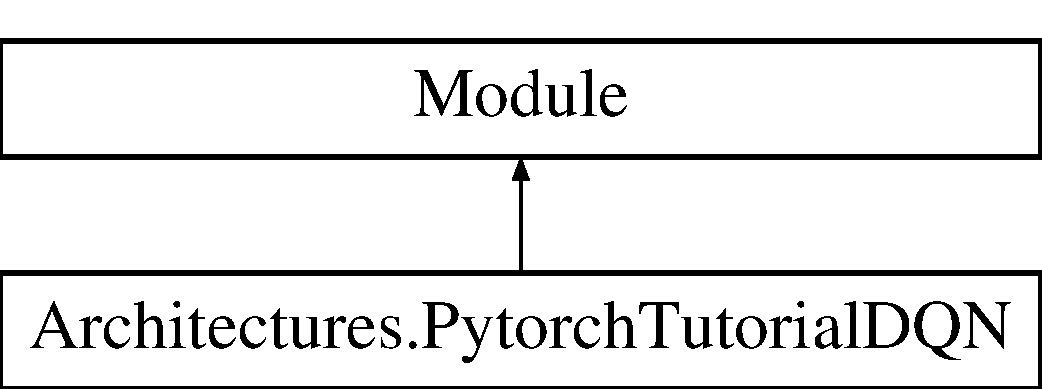
\includegraphics[height=2.000000cm]{classArchitectures_1_1PytorchTutorialDQN}
\end{center}
\end{figure}
\subsection*{Public Member Functions}
\begin{DoxyCompactItemize}
\item 
\mbox{\Hypertarget{classArchitectures_1_1PytorchTutorialDQN_a8fa868705cc5d85d07c91643df260c60}\label{classArchitectures_1_1PytorchTutorialDQN_a8fa868705cc5d85d07c91643df260c60}} 
def {\bfseries \+\_\+\+\_\+init\+\_\+\+\_\+} (self, F\+L\+A\+GS)
\item 
\mbox{\Hypertarget{classArchitectures_1_1PytorchTutorialDQN_ad35305798200b012da272b95c07b1cd8}\label{classArchitectures_1_1PytorchTutorialDQN_ad35305798200b012da272b95c07b1cd8}} 
def {\bfseries forward} (self, screen)
\end{DoxyCompactItemize}
\subsection*{Public Attributes}
\begin{DoxyCompactItemize}
\item 
\mbox{\Hypertarget{classArchitectures_1_1PytorchTutorialDQN_a590482e613bb211334d3f9e53efd488b}\label{classArchitectures_1_1PytorchTutorialDQN_a590482e613bb211334d3f9e53efd488b}} 
{\bfseries xy\+\_\+space}
\item 
\mbox{\Hypertarget{classArchitectures_1_1PytorchTutorialDQN_aa7a1c5c0550d4b3e624c401a96648031}\label{classArchitectures_1_1PytorchTutorialDQN_aa7a1c5c0550d4b3e624c401a96648031}} 
{\bfseries conv1}
\item 
\mbox{\Hypertarget{classArchitectures_1_1PytorchTutorialDQN_ac3080bc1ac06f15c93e70416cde9fe41}\label{classArchitectures_1_1PytorchTutorialDQN_ac3080bc1ac06f15c93e70416cde9fe41}} 
{\bfseries bn1}
\item 
\mbox{\Hypertarget{classArchitectures_1_1PytorchTutorialDQN_a52f93b03f0804f5a4d7ff2277221e69d}\label{classArchitectures_1_1PytorchTutorialDQN_a52f93b03f0804f5a4d7ff2277221e69d}} 
{\bfseries conv2}
\item 
\mbox{\Hypertarget{classArchitectures_1_1PytorchTutorialDQN_ac02c20ec076eb7a24ad3d0440238e431}\label{classArchitectures_1_1PytorchTutorialDQN_ac02c20ec076eb7a24ad3d0440238e431}} 
{\bfseries bn2}
\item 
\mbox{\Hypertarget{classArchitectures_1_1PytorchTutorialDQN_abb39d47e8d979fb70f09135131468e92}\label{classArchitectures_1_1PytorchTutorialDQN_abb39d47e8d979fb70f09135131468e92}} 
{\bfseries conv3}
\item 
\mbox{\Hypertarget{classArchitectures_1_1PytorchTutorialDQN_a7b509e099d0860a7275370644b2ecd2e}\label{classArchitectures_1_1PytorchTutorialDQN_a7b509e099d0860a7275370644b2ecd2e}} 
{\bfseries bn3}
\item 
\mbox{\Hypertarget{classArchitectures_1_1PytorchTutorialDQN_a6f8d4bf1ed2376571ee2d46b0186421c}\label{classArchitectures_1_1PytorchTutorialDQN_a6f8d4bf1ed2376571ee2d46b0186421c}} 
{\bfseries conv4}
\item 
\mbox{\Hypertarget{classArchitectures_1_1PytorchTutorialDQN_a0b3d86d48066c3c4a36a4a3f829ace9c}\label{classArchitectures_1_1PytorchTutorialDQN_a0b3d86d48066c3c4a36a4a3f829ace9c}} 
{\bfseries bn4}
\item 
\mbox{\Hypertarget{classArchitectures_1_1PytorchTutorialDQN_af8af6c9a79216639cf0f6fb77b2d6c2f}\label{classArchitectures_1_1PytorchTutorialDQN_af8af6c9a79216639cf0f6fb77b2d6c2f}} 
{\bfseries tmp\+\_\+w}
\item 
\mbox{\Hypertarget{classArchitectures_1_1PytorchTutorialDQN_ae15c6d063adff1f55b087bb5d2bcdb50}\label{classArchitectures_1_1PytorchTutorialDQN_ae15c6d063adff1f55b087bb5d2bcdb50}} 
{\bfseries fc1}
\item 
\mbox{\Hypertarget{classArchitectures_1_1PytorchTutorialDQN_a1ecd5afb1fcf257b2e01919fa54c6d07}\label{classArchitectures_1_1PytorchTutorialDQN_a1ecd5afb1fcf257b2e01919fa54c6d07}} 
{\bfseries head\+\_\+actions}
\end{DoxyCompactItemize}


\subsection{Detailed Description}
Documentation for \mbox{\hyperlink{classArchitectures_1_1PytorchTutorialDQN}{Pytorch\+Tutorial\+D\+QN}}. 

More details. 

The documentation for this class was generated from the following file\+:\begin{DoxyCompactItemize}
\item 
Architectures.\+py\end{DoxyCompactItemize}

\hypertarget{classAgency_1_1ReplayBuffer}{}\section{Agency.\+Replay\+Buffer Class Reference}
\label{classAgency_1_1ReplayBuffer}\index{Agency.\+Replay\+Buffer@{Agency.\+Replay\+Buffer}}


Documentation for \mbox{\hyperlink{classAgency_1_1ReplayBuffer}{Replay\+Buffer}}.  


Inheritance diagram for Agency.\+Replay\+Buffer\+:\begin{figure}[H]
\begin{center}
\leavevmode
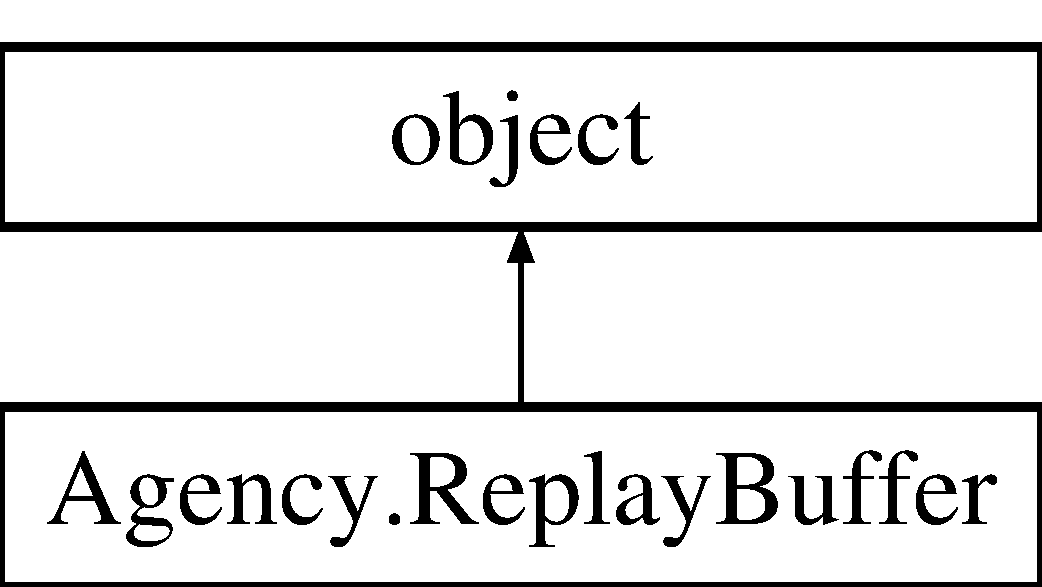
\includegraphics[height=2.000000cm]{classAgency_1_1ReplayBuffer}
\end{center}
\end{figure}
\subsection*{Public Member Functions}
\begin{DoxyCompactItemize}
\item 
\mbox{\Hypertarget{classAgency_1_1ReplayBuffer_ae1d76f1730f31d4fa36c7f7490e7fa2c}\label{classAgency_1_1ReplayBuffer_ae1d76f1730f31d4fa36c7f7490e7fa2c}} 
def {\bfseries \+\_\+\+\_\+init\+\_\+\+\_\+} (self, capacity)
\item 
\mbox{\Hypertarget{classAgency_1_1ReplayBuffer_a7792c36c85702b20aadfd91ec4c4326f}\label{classAgency_1_1ReplayBuffer_a7792c36c85702b20aadfd91ec4c4326f}} 
def {\bfseries \+\_\+\+\_\+len\+\_\+\+\_\+} (self)
\item 
\mbox{\Hypertarget{classAgency_1_1ReplayBuffer_ad6b534eb2f5e5d14a19504c543a061ac}\label{classAgency_1_1ReplayBuffer_ad6b534eb2f5e5d14a19504c543a061ac}} 
def {\bfseries \+\_\+\+\_\+getitem\+\_\+\+\_\+} (self, key)
\item 
def \mbox{\hyperlink{classAgency_1_1ReplayBuffer_a42eb421de8a87af670f58c2c9f47819c}{push}} (self, args)
\item 
def \mbox{\hyperlink{classAgency_1_1ReplayBuffer_ad4826e3b32056d091daed1120862760c}{sample}} (self, batch\+\_\+size)
\end{DoxyCompactItemize}
\subsection*{Public Attributes}
\begin{DoxyCompactItemize}
\item 
\mbox{\Hypertarget{classAgency_1_1ReplayBuffer_aa7be9fdc4ca2207005cb997ecd16cefe}\label{classAgency_1_1ReplayBuffer_aa7be9fdc4ca2207005cb997ecd16cefe}} 
{\bfseries capacity}
\item 
\mbox{\Hypertarget{classAgency_1_1ReplayBuffer_aabee82626e7bdea8a188ae1fd7783430}\label{classAgency_1_1ReplayBuffer_aabee82626e7bdea8a188ae1fd7783430}} 
{\bfseries memory}
\item 
\mbox{\Hypertarget{classAgency_1_1ReplayBuffer_a74ddbf1602593e4d1de547773c61a67c}\label{classAgency_1_1ReplayBuffer_a74ddbf1602593e4d1de547773c61a67c}} 
{\bfseries position}
\item 
\mbox{\Hypertarget{classAgency_1_1ReplayBuffer_a3472d419a502e3331128f223253d4a78}\label{classAgency_1_1ReplayBuffer_a3472d419a502e3331128f223253d4a78}} 
{\bfseries Transition}
\end{DoxyCompactItemize}


\subsection{Detailed Description}
Documentation for \mbox{\hyperlink{classAgency_1_1ReplayBuffer}{Replay\+Buffer}}. 

More details. \begin{DoxyVerb}Experience Replay Buffer Class \end{DoxyVerb}
 

\subsection{Member Function Documentation}
\mbox{\Hypertarget{classAgency_1_1ReplayBuffer_a42eb421de8a87af670f58c2c9f47819c}\label{classAgency_1_1ReplayBuffer_a42eb421de8a87af670f58c2c9f47819c}} 
\index{Agency\+::\+Replay\+Buffer@{Agency\+::\+Replay\+Buffer}!push@{push}}
\index{push@{push}!Agency\+::\+Replay\+Buffer@{Agency\+::\+Replay\+Buffer}}
\subsubsection{\texorpdfstring{push()}{push()}}
{\footnotesize\ttfamily def Agency.\+Replay\+Buffer.\+push (\begin{DoxyParamCaption}\item[{}]{self,  }\item[{}]{args }\end{DoxyParamCaption})}

\begin{DoxyVerb}store transition in replay buffer \end{DoxyVerb}
 \mbox{\Hypertarget{classAgency_1_1ReplayBuffer_ad4826e3b32056d091daed1120862760c}\label{classAgency_1_1ReplayBuffer_ad4826e3b32056d091daed1120862760c}} 
\index{Agency\+::\+Replay\+Buffer@{Agency\+::\+Replay\+Buffer}!sample@{sample}}
\index{sample@{sample}!Agency\+::\+Replay\+Buffer@{Agency\+::\+Replay\+Buffer}}
\subsubsection{\texorpdfstring{sample()}{sample()}}
{\footnotesize\ttfamily def Agency.\+Replay\+Buffer.\+sample (\begin{DoxyParamCaption}\item[{}]{self,  }\item[{}]{batch\+\_\+size }\end{DoxyParamCaption})}

\begin{DoxyVerb}return random sample transition from ER \end{DoxyVerb}
 

The documentation for this class was generated from the following file\+:\begin{DoxyCompactItemize}
\item 
Agency.\+py\end{DoxyCompactItemize}

%--- End generated contents ---

% Index
\backmatter
\newpage
\phantomsection
\clearemptydoublepage
\addcontentsline{toc}{chapter}{Index}
\printindex

\end{document}
